\section{Methods}
%describe the methods, the data, the assumptions, the scenarios, a brief few 
%sentences on Temoa itself.
This work collected data from multiple sources to populate a model of the 
Illinois electric grid. This simulated representation of the state of 
Illinois relies on the Temoa framework, an open source tool built by the North 
Carolina State University that enables energy system optimization and 
techno-economic analysis 
\cite{decarolis_temoa_2010,decarolis_modelling_2016,decarolis_formalizing_2017}.

\subsection{Optimization Analysis}
This work established optimal solutions to 
various scenarios which illuminate the potential impact of nuclear plant 
closures and other policy options on the cost of power in Illinois. These 
simulations  also explore the state of Illinois' ability to meet its aggressive 
carbon goals with and without maintenance and expansion of nuclear power 
capacity. 

Assumptions and constraints in these simulations differentiate the scenarios 
presented here. Each optimized scenario is the solution to a linear programming 
problem  comprised of two key components. First, the objective function in this case 
minimizes the total system cost of the energy grid in the state of Illinois. 
Second, a set of constraints limit the model soluations. Then, optimization 
proceeds by varying all free parameters within the scope of the defined constraints in order 
to meet the objective.

In this case, Temoa varies the deployed ratio of generation technologies on the 
Illinois electric grid, within the constraints of various policies, to minimize 
cost. The simulations each begin in the year 2020 
and proceed through 2050. The initial condition in 2020 represents the current 
electricity generation mix in the state of Illinois today.


\subsection{Data}
% paragraph on data sources
Data sources for this model of Illinois included multiple national and regional 
databases. Primarily this work relied on federal and international databases from the 
Energy Information Administration 
\cite{us_energy_information_administration_eia_preliminary_2021,energy_information_administration_state_2020,us_energy_information_administration_eia_electric_2021,us_energy_information_administration_eia_illinois_2020}, 
the U.S. Geological Survey \cite{hoen_united_2018}, 
International Energy Agency \cite{lorenczik_projected_2020}, 
the Nuclear Energy Agency \cite{crozat_full_2018}
, the Nuclear Regulatory Commission \cite{united_states_nuclear_regulatory_commission_illinois_2020}, 
the Intergovernmental Panel on Climate Change 
\cite{intergovernmental_panel_on_climate_change_annex_2014,intergovernmental_panel_on_climate_change_climate_2014,intergovernmental_panel_on_climate_change_climate_2014-1,intergovernmental_panel_on_climate_change_climate_2014-2}
the Interstate Renewable Energy Council 
\cite{sherwood_us_2009,sherwood_us_2010,sherwood_us_2011,brown_solid_1996,sherwood_us_2012,sherwood_us_2013,sherwood_us_2014}
and the Department of Energy's EERE and NE offices 
\cite{us_department_of_energy_capital_2016}, the National Renewable Energy 
Laboratory \cite{nrel_national_renewable_energy_laboratory_2020_2020}.
Industry sources included the World Nuclear Association
\cite{world_nuclear_association_nuclear_2017}
, 
the Nuclear Energy Institute 
\cite{desai_nuclear_2018,desai_nuclear_2020,murphy_impacts_2019,tessum_air_2019},
Rockland Capital Generation \cite{rockland_capital_natural_2021},
Sargent \& Lundy \cite{sargent__lundy_capital_2020}, 
Lazard \cite{ray_lazards_2020},
and others 
\cite{the_solar_foundation_national_2020,solar_energy_industries_association_illinois_2020,rutovitz_calculating_2015}.


% paragraph on reproducibility and location of data/analysis
This work was conducted in the open under a BSD-3 open-source license by the 
Advanced Reactors and Fuel Cycles group at the University of Illinois. The 
data, models, and assumptions used in his work can all be found and explored at 
open source repository at 
\href{https://github.com/arfc/2021-04-nm-illinois}{github.com/arfc/2021-04-nm-illinois}.


\section{Scenarios Simulated}\label{sec:simulations}

This model of Illinois' electric generation leverages robust data and populates 
an open-source framework for simulating and optimizing energy systems, 
the Temoa framework (Tools for Energy Model Optimization and Analysis). 
In this work 

we are able to determine the optimal energy generation mix 
for the UIUC microgrid for various objective functions (minimize carbon, 
minimize cost, etc.) while meeting system constraints (zero carbon by 2050, 
practical deployment speeds, realistic improvements in storage technology 
capabilities, etc.). The UIUC microgrid model includes transportation as well 
as campus steam, electric, and chilled water demand and provides cross-decadal 
deployment solutions which optimize the scenario objective function (Figure 2).

This model is underpinned by multiple advanced techniques. For example, a 
predictive model of net electricity demand on campus has been created with an 
echo state network machine learning approach to generate representative 
synthetic predictions of net grid load (Figure 3). This predictive model 
incorporates weather information to account for solar and wind power generation 
as well as heating and air-conditioning demands. Such predictive models are 
trained using multi-year historic campus electricity generation and consumption 
data. A similar approach will be used in the proposed simulations of the state 
as a whole.

\subsection{Generated Waste Data}
***description of waste calculator notebook for nuclear/wind/solar***

Coal power plants primarily produce solid wastes in the form of ash and slurries from the scrubbers.  Coal ash is produced from coal burning in approximately a 6:1 burned coal:coal ash ratio.  While the solid wastes are comprised of multiple elements, the waste is generally half coal ash, and half anhydrite ($CaSO_4$) - a product of chemical reactions in the scrubbers \cite{brown_solid_1996}.

\begin{figure}[h!]
\centering
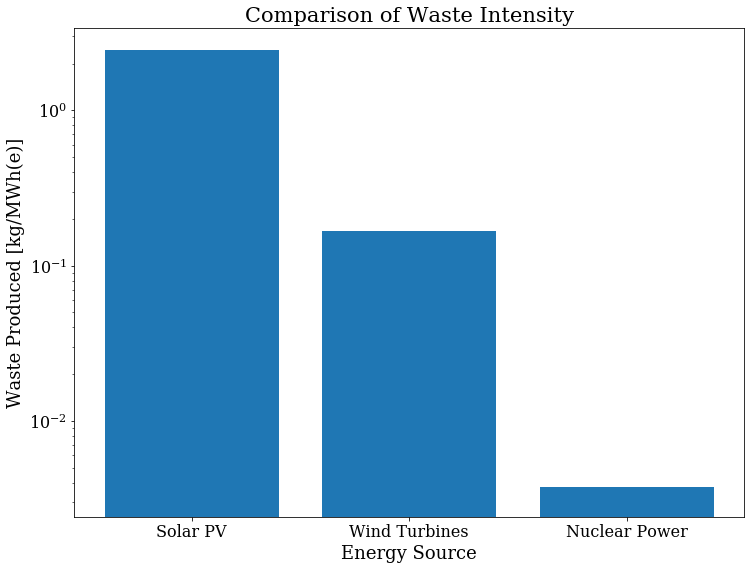
\includegraphics[width = 10cm]{img/mass-waste-intensity.png}
\caption{Solid Waste in $\frac{kg}{MWh}$ by Energy Source}
\label{fig:mass-waste}
\end{figure}



